%
%
%   Band VIII, 3 N.~??A25
%   Signatur/Tex-Datei: LH_35_13_03_203
%   RK-Nr. 58290
%   Überschrift: Tuba stentorea vel acustica [früher: Ad tubam stentoream vel acusticam]
%   Datierung: [1672 -- erste Hälfte 1685 (?)]
%   WZ: (keins)
%   SZ: (keins)
%   Bilddateien LH_35_13_03_203_d (insgesamt: eine)
%
%
\begin{ledgroupsized}[r]{120mm}
\footnotesize
%
\count\Bfootins=400
\count\Afootins=1200
\count\Cfootins=1200
\pstart
\noindent\textbf{Überlieferung:}
\pend
\end{ledgroupsized}
\begin{ledgroupsized}[r]{114mm}
\footnotesize
\pstart \parindent -6mm
\makebox[6mm][l]{\textit{L}}%
Aufzeichnung: LH~XXXV~13,~3 Bl.~203.
Ein Blatt~4\textsuperscript{o}.
Eineinhalb Seiten.
% Kein Was\-ser\-zei\-chen.
\pend
\end{ledgroupsized}
%
\vspace*{5mm}
\begin{ledgroup}
\footnotesize
\pstart
\noindent\textbf{Datierungsgründe:}
Das von S.~Morland\protect\index{Namensregister}{\textso{Morland} (Moreland), Samuel 1625\textendash1695} entwickelte Sprachrohr erwähnt Leibniz bereits in einer Notiz aus dem Jahre 1671 (\textit{LSB} VIII,~1 N.~58\cite{01277}).
Später hat er auch Morlands Abhandlung % über das Sprachrohr S.~\textsc{Morland}, 
\textit{Tuba stentoro-phonica} % an instrument of excellent use, as well at sea, as at land; invented and variously experimented in the year 1670, 
(London 1672\cite{00149}) gelesen,
wie Streichungen in seinem Handexemplar bezeugen (\textit{LSB} VIII,~1 N.~62\cite{01278}; vgl. Hannover, GWLB, Signatur N\textendash A 7073).
Auf die \textit{tuba stentorea} bezieht sich Leibniz auch in N.~12\textsubscript{3}, Textschicht \textit{Lil} (S.~\refpassage{LH_37_01_008v_tubastentorea-1}{LH_37_01_008v_tubastentorea-2}) % , sowie in N.~??X\textsubscript{7} (S.~\refpassage{LH_37_01_025v_tubastentorea-1}{LH_37_01_025v_tubastentorea-2}),
und zwar % beidemal 
in einem Kontext, der die Gestalt des Sprachrohrs in den Vordergrund stellt.
N.~12\textsubscript{3}, Textschicht \textit{Lil} % , und N.~??X\textsubscript{7} lassen 
lässt sich auf die Zeitspanne zwischen der zweiten Hälfte 1684 und der ersten Hälfte 1685 datieren.
Das vorliegende Stück N.~2 ist mit der Frage befasst, wie das Profil des Sprachrohrs im Hinblick auf eine handwerkliche Ausführung geometrisch zu gestalten ist.
Daher ist wahrscheinlich, dass N.~2 nach der Veröffentlichung von Morlands Abhandlung (1672), aber noch vor N.~12\textsubscript{3}, Textschicht \textit{Lil} % , und N.~??X\textsubscript{7} 
verfasst wurde.
Eine spätere Entstehungszeit ist jedoch nicht auszuschließen.
% Kein Wasserzeichen.\\
% Probsts Datierung: ab 1676 ?\\
\pend
\end{ledgroup}
%
\vspace*{8mm}
\pstart\noindent
\normalsize
%
\lbrack203~r\textsuperscript{o}\rbrack\ \edtext{Ad Tubam}{%
\lemma{Ad}\Bfootnote{%
\textit{(1)}~Tubicam
\textit{(2)}~Tubam%
~\textit{L}}}
%
stentoream\protect\index{Sachverzeichnis}{tuba stentorea} vel acusticam\protect\index{Sachverzeichnis}{tuba acustica}
%\edtext{\textit{ABEFI}}{%
%\lemma{\textit{ABEFI}}\Bfootnote{%
%\textit{erg.~L}}}
\edtext{\textit{ABEFI}}{%
{\lemma{\textit{ABEFI}}\Bfootnote{%
\textit{erg.~L}}}%
{\lemma{\textit{ABEFI}}\Cfootnote{%
Siehe das Diagramm \lbrack\textit{Fig.~1}\rbrack\ auf S.~\pageref{LH_35_13_03_203r_Fig.1}.}}}
formandam ab
\edtext{artifice,\protect\index{Sachverzeichnis}{artifex}
ut scilicet sectionem Tubae\protect\index{Sachverzeichnis}{sectio tubae}
in plano datam superficie cava\protect\index{Sachverzeichnis}{superficies cava} exhibeat,
considerari potest curvam\protect\index{Sachverzeichnis}{curva} \lbrack\textit{AB}\rbrack\ vel \textit{IF,}
cujus revolutione\protect\index{Sachverzeichnis}{revolutio curvae}}{%
\lemma{artifice}\Bfootnote{%
\textit{(1)}~, considerandum et,
\textit{(2)}~, ut scilicet \lbrack...\rbrack\ considerari potest
\textit{(a)}~curvae
\textit{(aa)}~cujus revolu
\textit{(bb)}~\textit{ABC,}
\textit{(b)}~curvam \textbar~\textit{AC} \textit{ändert Hrsg.}~\textbar\ vel \textit{IF,} cujus revolutione%
~\textit{L}}}
%
circa axem\protect\index{Sachverzeichnis}{axis} \textit{LM} superficies
\edtext{describitur,
ut constantem}{%
\lemma{describitur,}\Bfootnote{%
\hspace{-0,5mm}\textbar~considerari posse \textit{streicht Hrsg.}~\textbar\
ut constantem%
\textit{~L}}}
%
ex rectis \textit{BC}, \textit{CD} etc.
\edtext{vel \textit{FG}, \textit{GH} etc.}{%
\lemma{vel}\Bfootnote{% \hspace*{-0,5mm}
\textit{FG}, \textit{GH}, etc.
\textit{erg.~L}}}
%
quae productae occurrant Axi,\protect\index{Sachverzeichnis}{axis}
nempe \textit{BC}
\edtext{in \textit{N}, vel \textit{CD} in \lbrack\textit{P}\rbrack,}{%
\lemma{in}\Bfootnote{%
\hspace{-0,5mm}\textit{N},
\textit{(1)}~et \textit{P}
\textit{(2)}~vel \textit{CD} in \textbar~\textit{B} \textit{ändert Hrsg.}~\textbar~,%
~\textit{L}}}
%
et ita porro.
Itaque \textit{BC}
\edtext{est portio truncata superficiei}{%
\lemma{est}\Bfootnote{%
\textit{(1)}~superficies
\textit{(2)}~portio truncata superficiei%
~\textit{L}}}
%
coni \textit{NCB},\protect\index{Sachverzeichnis}{conus}
et \textit{DC} coni
\edlabel{LH_35_13_03_203r_iduds-1}\textit{PDC}.%
\edtext{}{%
{\xxref{LH_35_13_03_203r_iduds-1}{LH_35_13_03_203r_iduds-2}}%
{\lemma{\textit{PDC}.}\Bfootnote{%
\textit{(1)}~Jam superficies conica
\textit{(2)}~Res ergo \lbrack...\rbrack\ superficies conica
\textit{(a)}~, quod fiet
\textit{(b)}~. Hoc ut fiat%
~\textit{L}}}}
%
\pend
%
\pstart
Res ergo huc redit ut plana lamina\protect\index{Sachverzeichnis}{lamina plana} exhibeatur,
ex qua formari possit superficies\protect\index{Sachverzeichnis}{superficies conica} conica.
Hoc ut fiat\edlabel{LH_35_13_03_203r_iduds-2}
demonstrativa ratione\protect\index{Sachverzeichnis}{ratio demonstrativa}
\edtext{consideravi\lbrack:\rbrack\
ut cylindrica superficies\protect\index{Sachverzeichnis}{superficies cylindrica}}{%
\lemma{consideravi}\Bfootnote{%
\textit{(1)}~sup
\textit{(2)}~conicam super
\textit{(3)}~ut cylindrica superficies%
~\textit{L}}}
%
plano applicari potest volvendo eam super plano,
et ita exhibendo planum superficiei congruens;\protect\index{Sachverzeichnis}{planum superficiei congruens}
\makebox[1.0\textwidth][s]{ita similiter conicam\protect\index{Sachverzeichnis}{superficies conica} quoque posse volvendo successive applicari plano
et ita exprimere}
\pend
\newpage
 \centerline{\includegraphics[width=0.51\textwidth]{gesamttex/edit_VIII,3/images/LH_35_13_03_203_d.pdf}}%
 \vspace{0.5em}
  \centerline{\lbrack\textit{Fig.~1}\rbrack}%
  \vspace{1.5em}
\pstart
\noindent 
%%%%    !!!!    !!!!    ACHTUNG GETRIXT    !!!!    !!!!
\label{LH_35_13_03_203r_Fig.1}\edtext{}{\lemma{\hspace*{1,6mm}\lbrack\textit{Fig.~1}\rbrack}\killnumber\Cfootnote{
Ein auf Bl.~203~r\textsuperscript{o} befindlicher, gestrichener Entwurf zum Diagramm wird nicht wiedergegeben.}}in plano magnitudinis suae vestigium,\protect\index{Sachverzeichnis}{vestigium magnitudinis}
prorsus ut circumferentia rotae\protect\index{Sachverzeichnis}{circumferentia rotae} plano
\edtext{applicatur.
Utrobique enim sive conus\protect\index{Sachverzeichnis}{conus}
sive cylinder\protect\index{Sachverzeichnis}{cylinder} volvatur,
superficies ejus tangit planum in recta.
Et sane si pro curva\protect\index{Sachverzeichnis}{curva}
figura adhibeatur polyhedrica curvae appropinquans,\protect\index{Sachverzeichnis}{figura polyhedrica curvae appropinquans}
tunc utique superficies polyhedra\protect\index{Sachverzeichnis}{superficies polyhedra}
magnitudinem\protect\index{Sachverzeichnis}{magnitudo superficiei} suam exprimeret in plano.
Id vero tantum hic in\-ter\-est inter conum\protect\index{Sachverzeichnis}{conus} et cylindrum;\protect\index{Sachverzeichnis}{cylinder}
quod}{%
\lemma{applicatur.}\Bfootnote{%
\textit{(1)}~Sed hoc interest inter coni et cylindri volutionem in plano quod
\textit{(2)}~Utrobique enim
\textit{(a)}~recta
\textit{(b)}~superficies planum
\textit{(aa)}~recta
\textit{(bb)}~tangit in recta
\textit{(c)}~sive conus \lbrack...\rbrack\ in recta % sive cylinder volvatur superficies ejus tangit planum
\textit{(aa)}~, et
\textit{(bb)}~. Et
\textbar~sane \textit{erg.}~%
\textbar\ si pro curva figura
\textbar~adhibeatur \textit{erg.}~%
\textbar\ polyhedrica
\textit{(aaa)}~pro
\textit{(bbb)}~\textbar~curvae \textit{erg.}~\textbar\ appropinquans,
\textit{(aaaa)}~adhibetur
\textit{(bbbb)}~tunc utique superficies
\textit{(aaaaa)}~polyhedrica
\textit{(bbbbb)}~polyhedra
\textit{(aaaaa-a)}~in plano
\textit{(bbbbb-b)}~de figu
\textit{(ccccc-c)}~su
\textit{(ddddd-d)}~magnitudinem suam \lbrack...\rbrack\ vero tantum % exprimeret in plano. Id
\textbar~hic \textit{erg.}~%
\textbar\ interest
\textit{(aaaaa-aa)}~,
\textit{(bbbbb-bb)}~inter conum et cylindrum; quod%
~\textit{L}}}
% % % %    < < < < 
in volutione cylindri\protect\index{Sachverzeichnis}{volutio cylindri}
rectae planum tangentes\protect\index{Sachverzeichnis}{recta tangens} sibi parallelae sunt,
in volutione vero coni\protect\index{Sachverzeichnis}{volutio coni} concurrunt
in apice\protect\index{Sachverzeichnis}{apex coni} coni. 
\pend
%
\pstart
Hoc posito sequitur\lbrack:\rbrack\
si ex puncto \textit{N}, tanquam apice\protect\index{Sachverzeichnis}{apex coni}
\edtext{coni, radio\protect\index{Sachverzeichnis}{radius circuli} \textit{NB} describatur}{%
\lemma{coni,}\Bfootnote{%
\textit{(1)}~describatur 
\textit{(2)}~radio \textit{NB} describatur%
~\textit{L}}}
%
\edtext{arcus\protect\index{Sachverzeichnis}{arcus circuli}
\lbrack\textit{RB\pgrk{G}FS}\rbrack\
vel \textit{RBS}}{%
\lemma{arcus}\Bfootnote{%
\textit{(1)}~\textit{BRF}
\textit{(2)}~\textbar~\textit{RBE\pgrk{G}FS} \textit{ändert Hrsg.}~\textbar\ vel
\textit{(a)}~\textit{RPF}
\textit{(b)}~\textit{RBS}%
~\textit{L}}}
%
aequalis circumferentiae\protect\index{Sachverzeichnis}{circumferentia circuli} circuli \textit{BEF}
\edtext{circa diametrum \textit{BF};}{%
\lemma{circa}\Bfootnote{%
\hspace{-0,5mm}diametrum \textit{BF}
\textit{erg.~L}}}
%
et similiter si radio \textit{NC} describatur arcus \textit{TCV}
aequalis curcumferentiae circuli circa diametrum\protect\index{Sachverzeichnis}{diameter circuli} \textit{CG},
fore portionem\protect\index{Sachverzeichnis}{portio annularis} annularem \textit{TRBSVCT}
aequalem superficiei\protect\index{Sachverzeichnis}{superficies conica}
\edtext{conicae truncatae
\lbrack\textit{CBEFG\pgrk{D}C},\rbrack}{%
\lemma{conicae}\Bfootnote{%
\textit{(1)}~\textit{CBEFG\pgrk{D}C}
\textit{(2)}~truncatae \textbar~\textit{GBEFG\pgrk{D}E}, \textit{ändert Hrsg.}~\textbar%
~\textit{L}}}
%
cujus superior basis est circumferentia circa \textit{CG},
inferior circumferentia\protect\index{Sachverzeichnis}{circumferentia circuli} circa \textit{BF}.
Patet
\edtext{autem puncta \textit{R}, \textit{T}, \textit{N} vel}{%
\lemma{autem}\Bfootnote{%
\textit{(1)}~\textit{R}, \textit{N}, \textit{T}
\textit{(2)}~\textit{RTN}
\textit{(3)}~puncta \textit{R}, \textit{T}, \textit{N} vel%
~\textit{L}}}
%
\textit{S}, \textit{V}, \textit{N} cadere in eandem
\edtext{rectam.
Quaeritur}{%
\lemma{rectam.}\Bfootnote{%
\textit{(1)}~Si
\textit{(2)}~Ut
\textit{(3)}~Quaeritur%
~\textit{L}}}
%
ergo tantum apertura\protect\index{Sachverzeichnis}{apertura coni}
seu angulus\protect\index{Sachverzeichnis}{angulus} \textit{RNS},
seu a dato circulo
(\phantom)\hspace*{-1.2mm}%
centro\protect\index{Sachverzeichnis}{centrum circuli} \textit{N} radio\protect\index{Sachverzeichnis}{radius circuli} \textit{NB} descripto%
\phantom(\hspace*{-1.2mm})
abscindere
\edtext{\textit{RBFS}}{%
\lemma{\textit{RBFS}}\Bfootnote{%
\textit{erg.~L}}}
%
arcum\protect\index{Sachverzeichnis}{arcus circuli} datae magnitudinis
seu aequalem circumferentiae\protect\index{Sachverzeichnis}{circumferentia circuli} datae
circa diametrum\protect\index{Sachverzeichnis}{diameter circuli} datam
\edlabel{LH_35_13_03_203r_ieuvg-3}\textit{BF}.
\edtext{}{%
{\xxref{LH_35_13_03_203r_ieuvg-3}{LH_35_13_03_203r_ieuvg-4}}%
{\lemma{\textit{BF}}\Bfootnote{%
\textit{(1)}~id est
\textit{(2)}~\textbar~. Hoc ita fiet, cum detur circumferentia integra per \textit{R}, \textit{B}, \textit{F}, \textit{S}, itemque arcus magnitudo seu circumf. per \textit{B}, \textit{E}, \textit{F}, dabitur et circumferentiarum ratio ea sc. quae diametrorum, ea sc. quae est anguli \textit{RNS} ad gradus 360. Ergo fiet ut recta \textit{NR} ad rectam \textit{BF}, ita 360 ad numerum graduum anguli \textit{NRS}.
\textit{streicht Hrsg.}~\textbar\
\lbrack203~v\textsuperscript{o}\rbrack\
\textit{(3)}~. Hoc ita fiet, cum detur
\textbar\ magnitudine \textit{erg. u. gestr.}~\textbar\ circumferentia integra per \textit{R}, \textit{B}, \textit{F}, \textit{S},
\textit{(a)}~tendens
\textit{(b)}~itemque magnitudo \lbrack...\rbrack\ diametrum \textit{BF}
\textit{(aa)}~\textbar~. Dabitur \textit{streicht Hrsg.}~\textbar\
\textit{(bb)}~, dabitur et ratio harum
\textit{(aaa)}~quantitatum
\textit{(bbb)}~circumferentiarum, eadem \lbrack...\rbrack\ graduum anguli % %%%%
\textit{(aaaa)}~\textit{NBF}
\textit{(bbbb)}~\textit{BNF},
\textit{(cccc)}~\textit{RNS}, ergo
\textit{(aaaaa)}~\textbar~ut \textit{streicht Hrsg.}~\textbar\
\textit{(aaaaa-a)}~diam
\textit{(bbbbb-b)}~\textit{NB} ad \textit{MB}
\textit{(bbbbb)}~ut \textit{NB} \lbrack...\rbrack\ 360 ad % ad \textit{MB} ita erit
\textit{(aaaaa-a)}~gradus \textbar~anguli \textit{streicht Hrsg.}~\textbar\ \textit{BNF}, qui
\textit{(bbbbb-b)}~numerum graduum \lbrack...\rbrack\ numerus desiderabatur. % anguli \textit{RNS}, qui
\textit{(aaaaa-aa)}~Eodem
\textit{(bbbbb-bb)}~Unde etiam
\textit{(ccccc-cc)}~Et eodem modo erit
\textit{(aaaaa-aaa)}~\textit{NT} ad \textit{TV} \textbar~(\phantom)\hspace*{-1.2mm}dimidiam \textit{CW}\phantom(\hspace*{-1.2mm}) \textit{erg.}~\textbar\ ut 360 ad numerum
\textit{(bbbbb-bbb)}~\textit{NC} ad \textit{CW}
\textit{(ccccc-ccc)}~\textit{NC} ad \textit{CW} (\phantom)\hspace*{-1.2mm}dimidiam \textbar~\textit{CV} \textit{ändert Hrsg.}~\textbar\ \phantom(\hspace*{-1.2mm}) ut
\textit{(aaaaa-aaaa)}~360 num
\textit{(bbbbb-bbbb)}~360 ad \lbrack...\rbrack\ anguli \textit{TNV} % numerum graduum
\textit{(aaaaa-aaaaa)}~. Sunt enim ob
\textit{(bbbbb-bbbbb)}~vel \textit{RNS}. \lbrack...\rbrack\ \textit{NB} ad \textit{BM}.% % ob triangula \textit{NWC}, \textit{NMB} similia est \textit{NC} ad \textit{CW}, ut
~\textit{L}}}}%
%
% \pend
%
% \pstart
%
\lbrack203~v\textsuperscript{o}\rbrack\ % Bl. 203v
%
% \pend
%
% \pstart
Hoc ita fiet,
cum detur circumferentia integra
per \textit{R}, \textit{B}, \textit{F}, \textit{S},
itemque magnitudo arcus \textit{B\pgrk{G}F},
aequalis circumferentiae integrae per \textit{B}, \textit{E}, \textit{F},
seu circa diametrum \textit{BF},
dabitur et ratio harum circumferentiarum,\protect\index{Sachverzeichnis}{circumferentia circuli}
eadem quae radiorum \textit{NB}, \textit{MB};
sed circumferentia integra per \textit{R}, \textit{B}, \textit{F}, \textit{S}
est ad partem suam,
arcum\protect\index{Sachverzeichnis}{arcus circuli} scilicet \textit{B\pgrk{G}F},
ut 360 gradus\protect\index{Sachverzeichnis}{gradus anguli} sunt ad numerum graduum anguli \textit{RNS},
ergo ut \textit{NB} ad \textit{MB}
ita erit 360 ad numerum graduum anguli \textit{RNS},
qui numerus desiderabatur.\protect\index{Sachverzeichnis}{numerus desideratus}
Et eodem modo erit \textit{NC} ad \textit{CW}
(\phantom)\hspace*{-1.2mm}%
dimidiam \lbrack\textit{CG}\rbrack%
\phantom(\hspace*{-1.2mm})
ut 360 ad numerum graduum anguli\protect\index{Sachverzeichnis}{gradus anguli} \textit{TNV} vel \textit{RNS}.
Nam ob triangula \textit{NWC}, \textit{NMB} similia,\protect\index{Sachverzeichnis}{triangulum simile}
est \textit{NC} ad \textit{CW},
ut \textit{NB} ad \textit{BM}.%
\edlabel{LH_35_13_03_203r_ieuvg-4}
%
Habito igitur angulo\protect\index{Sachverzeichnis}{angulus} \textit{BNF}, et
\edtext{radiis\protect\index{Sachverzeichnis}{radius circuli} \textit{NC}, \textit{NB},
\lbrack habetur et\rbrack}{%
\lemma{radiis}\Bfootnote{%
\textit{(1)}~\textit{BF}
\textit{(2)}~\textit{BN}, \textit{BT},
\textit{(3)}~\textit{NT}, \textit{NB}, habetur
\textit{(4)}~\textit{NC}, \textit{NB},
\textbar~habetur et \textit{erg. Hrsg.}~\textbar%
~\textit{L}}}
%
\edtext{descriptio portionis\protect\index{Sachverzeichnis}{portio annularis} annularis}{%
\lemma{descriptio}\Bfootnote{%
\textit{(1)}~figurae
\textit{(2)}~portionis annularis%
~\textit{L}}}
%
quaesitae.\protect\index{Sachverzeichnis}{descriptio quaesita}
\pend
\count\Bfootins=1000
\count\Afootins=1200
\count\Cfootins=1200
%
%
% ENDE DES STÜCKS AUF Bl. 203v
%
%
% \edtext{Hoc ita fiet,
% cum detur circumferentia integra per \textit{R}, \textit{B}, \textit{F}, \textit{S},
% itemque arcus magnitudo seu circumf. per \textit{B}, \textit{E}, \textit{F},
% dabitur et circumferentiarum ratio\lbrack,\rbrack\
% ea sc. quae diametrorum,
% ea sc. quae est anguli \textit{RNS} ad gradus 360.
% Ergo fiet\lbrack:\rbrack\ ut recta \textit{NR} ad rectam \textit{BF},
% ita 360 ad numerum graduum anguli \textit{NRS}.}{%
% \lemma{Hoc \lbrack...\rbrack\ \textit{NRS}}\Cfootnote{%
% Diese Textpassage hat Leibniz unmittelbar nach dem Umbruch von Bl.~203~r\textsuperscript{o} auf Bl.~203~v\textsuperscript{o} wiederholt und verändert.
% Siehe die folgenden Zeilen bis zum Textende.}}
%
%